\ExplSyntaxOn

\int_new:N \l__binp_int
\int_set:Nn \l__binp_int {4}
\tl_new:N \l__bina_tl
\tl_new:N \l__binb_tl
\tl_new:N \l__binhw_tl
\int_new:N \l__bina_int
\int_new:N \l__binb_int
\int_new:N \l__binc_int
\int_new:N \l__bind_int
\fp_new:N \l__bina_fp

\DeclareDocumentCommand \BinaryPrecision {m}
{
  \int_set:Nn \l__binp_int {#1}
}

\cs_new_nopar:Npn \int_to_bin:Nn #1#2
{
  \tl_clear:N #1
  \int_set:Nn \l__bina_int {#2}
  \prg_replicate:nn {\l__binp_int}
  {
    \int_set:Nn \l__binb_int {\int_mod:nn {\l__bina_int} {2}}
    \tl_put_left:Nx #1 {\int_use:N \l__binb_int}
    \int_set:Nn \l__bina_int {\int_div_truncate:nn {\l__bina_int} {2}}
  }
}

\cs_new_nopar:Npn \bin_hamming_weight:NN #1#2
{
  \tl_set_eq:NN \l__binhw_tl #2
  \tl_replace_all:Nnn \l__binhw_tl {0} {}
  \int_set:Nn #1 {\tl_count:N \l__binhw_tl}
}

\cs_new_nopar:Npn \bin_flip_one:NNn #1#2#3
{
  \tl_set_eq:NN #2#1
  \prg_replicate:nn {#3 - 1}
  {
    \tl_replace_once:Nnn #2 {1} {a}
  }
  \tl_replace_once:Nnn #2 {1} {0}
  \tl_replace_all:Nnn #2 {a} {1}
}

\DeclareDocumentCommand \HammingWeight {m m}
{
  \int_to_bin:Nn \l__binhw_tl {#2}
  \bin_hamming_weight:NN #1 \l__binhw_tl
}

\DeclareDocumentCommand \HyperCube {m}
{
  \int_set:Nn \l__binp_int {#1}
  \int_zero_new:c {l__hyper_0_int}
  \int_set:cn {l__hyper_0_int} {-1}
  \int_step_inline:nnnn {1} {1} {#1}
  {
    \int_zero_new:c {l__hyper_##1_int}
    \int_set:cn  {l__hyper_##1_int} {\int_use:c {l__hyper_\int_eval:n {##1 - 1}_int} * (#1 - ##1 + 1) / ##1}
  }
  \fp_set:Nn \l__bina_fp {2^{#1}-1}
  \int_set:Nn \l__binc_int {\fp_to_int:N \l__bina_fp}
  \int_step_inline:nnnn {0} {1} {\l__binc_int}
  {
    \int_to_bin:Nn \l__bina_tl {##1}
    \bin_hamming_weight:NN \l__binb_int \l__bina_tl
    \node[every~ hypercube~ label/.try] (hg- \l__bina_tl) at (\int_use:c {l__hyper_\int_use:N \l__binb_int _int},\int_use:N \l__binb_int) {\texttt{\l__bina_tl}};
    \int_incr:c {l__hyper_\int_use:N \l__binb_int _int}
    \int_incr:c {l__hyper_\int_use:N \l__binb_int _int}
  }
  \int_step_inline:nnnn {0} {1} {\l__binc_int}
    {
      \int_to_bin:Nn \l__bina_tl {##1}
      \bin_hamming_weight:NN \l__binb_int \l__bina_tl
      \int_step_inline:nnnn {1} {1} {\l__binp_int}
      {
        \bin_flip_one:NNn \l__bina_tl \l__binb_tl {####1}
        \tl_if_eq:NNTF \l__bina_tl \l__binb_tl
          { % do nothing if nodes are the same
          }
          {
            \draw[every~ hypercube~ edge/.try] (hg- \l__bina_tl) -- (hg- \l__binb_tl);
          }
      }
    }
  }

\ExplSyntaxOff

% Macro to cross out a single node
\newcommand{\CrossOutNode}[1]{%
  \draw[red, thick]
    ($(#1) + (-0.3, 0.3)$)
    --
    ($(#1) + (0.3, -0.3)$);
  \draw[red, thick]
    ($(#1) + (-0.3, -0.3)$)
    --
    ($(#1) + (0.3, 0.3)$);
}

% Macro to cross out a list of nodes
\newcommand{\CrossOutNodes}[1]{%
  \foreach \n in {#1} {%
    \CrossOutNode{\n}%
  }
}
% Macro to draw a circle around a single node
\newcommand{\CircleNode}[2][RoyalBlue]{%
  \draw[#1, thick]
    ($(#2)$)
    circle (0.5);
}

% Macro to circle a list of nodes
\newcommand{\CircleNodes}[2][RoyalBlue]{%
  \foreach \n in {#2} {%
    \CircleNode[#1]{\n}%
  }
}

% Überwachungstabelle der Aufgabe mit 10 Nachrichtenbits und 4 Kontrollbits
% (Spalten 1 bis 14, Zeilen c1 bis c4); Massstab im tikzpicture setzen
\newcommand{\ueberwachungZehnVier}{%
  \fill[blue!25] (0,0) rectangle (15,1);
  \fill[blue!15] (0,-4) rectangle (1,0);
  \fill[gray!8] (1,-4) rectangle (15,0);
  \foreach \i in {1,...,10} {
      \node at (\i+.5,.5) {\(a_{\i}\)};
    }
  \foreach \i in {1,...,4} {
      \pgfmathtruncatemacro{\col}{10+\i}
      \node[text=orange!80!black] at (\col+.5,.5) {\(c_{\i}\)};
      \node[text=orange!80!black] at (.5,.5-\i) {\(c_{\i}\)};
    }
  % Überwachungsbereiche von c1 bis c4, eine Liste pro Zeile
  \foreach \cols [count=\z] in {{1,2,3,5,6,7,11},{1,2,4,5,8,9,12},{1,3,4,6,8,10,13},{2,3,4,7,9,10,14}} {
      \foreach \col in \cols {
          \node at (\col+.5,.5-\z) {\(\times\)};
        }
    }
  % Trennung Nachrichtenbits / Kontrollbits
  \draw[blue!70!black,very thick] (11,-4) -- (11,1);
  \draw[step=1,black!30,thin] (0,-4) grid (15,1);
  \draw[black!65] (0,-4) rectangle (15,1);
}

% Bitwerte des Codeworts über den Spaltentiteln
% #1: 14 Bits als Komma-Liste, #2: Spalte magenta hervorheben (0 = keine)
\newcommand{\ueberwachungWerte}[2]{%
  \node[font=\small\itshape,anchor=east] at (1,1.5) {Wert};
  \foreach \w [count=\col] in {#1} {
      \ifnum\col=#2
        \node[magenta,font=\small\bfseries\ttfamily] at (\col+.5,1.5) {\w};
      \else
        \node[font=\small\ttfamily] at (\col+.5,1.5) {\w};
      \fi
    }
}

% Anzahl Einsen unter den Kreuzen jeder Zeile rechts der Tabelle,
% ungerade Anzahlen (Kontrollbit meldet) magenta
\newcommand{\ueberwachungEinsen}[1]{%
  \node[font=\small\itshape] at (16.4,.5) {Einsen};
  \foreach \n [count=\z] in {#1} {
      \ifodd\n
        \node[magenta] at (16.4,.5-\z) {\textbf{\n}\ \(\boldsymbol{\times}\)};
      \else
        \node[green!50!black] at (16.4,.5-\z) {\n\ \checkmark};
      \fi
    }
}


% command to make sure colorboxes don't create whitespace between code lines
\fboxsep=.6pt

% default settings for listings
\lstset{style=python}

\title[Datenintegrität]{Datenintegrität}

\subtitle{Optimale Codes und Hamming-Codes}

\author[Blum, Cyril] % (optional)
{Cyril Blum}

\institute[KLW] % (optional)
{
    Fachschaft Informatik\\
    Kantonsschule im Lee
}

\date[\today] % (optional)

\logo{\includegraphics[width=2cm]{Logos/FreeFlower.pdf}}

\titlegraphic{\vspace{-.7cm}\includegraphics[width=.85\textwidth]{"Grundlagen_Info/06_Datenbanken/Figures/title-emojis"}}

\frame{\titlepage}


% Beispiel für die ersten Folien: Nachricht 0101 1111 0010 1011 (wie beim Codieren weiter unten)
% Kartentrick-Codewort: a1..a16, dann c1..c9
\def\ktWerte{0,1,0,1,1,1,1,1,0,0,1,0,1,0,1,1,0,0,1,1,0,0,1,1,0}

% Kartentrick-Tabelle mit Beispielwerten; #1 = Nummer eines umgedrehten Nachrichtenbits (0 = keines)
\newcommand{\kartentrickGitter}[1]{%
    % Nachrichtenbits
    \foreach \r in {1,...,4} {
            \foreach \c in {1,...,4} {
                    \pgfmathtruncatemacro{\nr}{4*(\r-1)+\c}
                    \fill[gray!12] (\c-1,-\r) rectangle (\c,-\r+1);
                    \pgfmathtruncatemacro{\wert}{{\ktWerte}[\nr-1]}
                    \ifnum\nr=#1
                        \pgfmathtruncatemacro{\wert}{1-\wert}
                        \node[magenta] at (\c-.5,-\r+.5) {\texttt{\wert}};
                    \else
                        \node at (\c-.5,-\r+.5) {\texttt{\wert}};
                    \fi
                }
        }
    % Kontrollbits der Spalten (c1 bis c4) und der Zeilen (c5 bis c8)
    \foreach \c in {1,...,4} {
            \pgfmathtruncatemacro{\wert}{{\ktWerte}[15+\c]}
            \fill[blue!20] (\c-1,0) rectangle (\c,1);
            \node at (\c-.5,.5) {\texttt{\wert}};
        }
    \foreach \r in {1,...,4} {
            \pgfmathtruncatemacro{\wert}{{\ktWerte}[19+\r]}
            \fill[blue!20] (4,-\r) rectangle (5,-\r+1);
            \node at (4.5,-\r+.5) {\texttt{\wert}};
        }
    \fill[blue!20] (4,0) rectangle (5,1);
    \node at (4.5,.5) {\texttt{0}};
    \draw[step=1,black!65] (0,-4) grid (5,1);
}

% Überwachungstabelle der Kartentrick-Methode (16 Nachrichtenbits, 9 Kontrollbits)
\newcommand{\kartentrickUeberwachung}{%
    % Tabellenhintergrund
    \fill[blue!25] (0,0) rectangle (26,1);
    \fill[blue!15] (0,-9) rectangle (1,0);
    \fill[gray!8] (1,-9) rectangle (26,0);
    % Spalten- und Zeilenbeschriftung
    \foreach \i in {1,...,16} {
            \node at (\i+.5,.5) {\(a_{\i}\)};
        }
    \foreach \i in {1,...,9} {
            \pgfmathtruncatemacro{\col}{16+\i}
            \node at (\col+.5,.5) {\(c_{\i}\)};
            \node at (.5,.5-\i) {\(c_{\i}\)};
        }
    % c1 bis c4 überwachen die Spalten der Kartentrick-Tabelle
    \foreach \j in {1,...,4} {
            \foreach \r in {0,...,3} {
                    \pgfmathtruncatemacro{\col}{\j+4*\r}
                    \node at (\col+.5,.5-\j) {\(\times\)};
                }
        }
    % c5 bis c8 überwachen die Zeilen
    \foreach \r in {1,...,4} {
            \pgfmathtruncatemacro{\row}{\r+4}
            \foreach \j in {1,...,4} {
                    \pgfmathtruncatemacro{\col}{4*(\r-1)+\j}
                    \node at (\col+.5,.5-\row) {\(\times\)};
                }
        }
    % jedes Kontrollbit überwacht sich selbst
    \foreach \i in {1,...,8} {
            \pgfmathtruncatemacro{\col}{16+\i}
            \node at (\col+.5,.5-\i) {\(\times\)};
        }
    % c9 überwacht sämtliche Bits
    \foreach \col in {1,...,25} {
            \node at (\col+.5,-8.5) {\(\times\)};
        }
    \draw[step=1,black!30,thin] (0,-9) grid (26,1);
    \draw[black!65] (0,-9) rectangle (26,1);
}

% Zeile mit den Werten des Codeworts über der Tabelle; #1 = umgedrehtes Bit (0 = keines)
\newcommand{\kartentrickWertzeile}[1]{%
    \node[font=\scriptsize\itshape,anchor=east] at (1,1.5) {Wert};
    \foreach \col in {1,...,25} {
            \pgfmathtruncatemacro{\wert}{{\ktWerte}[\col-1]}
            \ifnum\col=#1
                \pgfmathtruncatemacro{\wert}{1-\wert}
                \node[magenta,font=\scriptsize\bfseries\ttfamily] at (\col+.5,1.5) {\wert};
            \else
                \node[font=\scriptsize\ttfamily] at (\col+.5,1.5) {\wert};
            \fi
        }
}


\begin{frame}{Rückblick: Kartentrick-Methode}
    Nachricht: \texttt{0101 1111 0010 1011}
    \begin{columns}
        \begin{column}{.4\textwidth}
            \begin{center}
                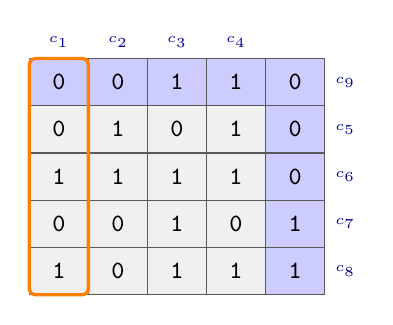
\begin{tikzpicture}[x=.75cm,y=.6cm,every node/.style={font=\small}]
                    \kartentrickGitter{0}
                    % Namen der Bits am Rand
                    \foreach \c in {1,...,4} {
                            \node[font=\tiny,blue!60!black] at (\c-.5,1.35) {\(c_{\c}\)};
                        }
                    \foreach \r in {1,...,4} {
                            \pgfmathtruncatemacro{\nr}{\r+4}
                            \node[font=\tiny,blue!60!black] at (5.35,-\r+.5) {\(c_{\nr}\)};
                        }
                    \node[font=\tiny,blue!60!black] at (5.35,.5) {\(c_9\)};
                    % Überwachungsbereich von c1
                    \draw<2->[orange,very thick,rounded corners=2pt] (0,-4) rectangle (1,1);
                \end{tikzpicture}
            \end{center}
        \end{column}
        \begin{column}{.55\textwidth}
            \begin{itemize}
                \item 16 Nachrichtenbits \(a_1, \ldots, a_{16}\) (zeilenweise), 9 Kontrollbits \(c_1, \ldots, c_9\)
                \item<2-> \(c_1\) überwacht die erste Spalte: \(a_1,a_5,a_9,a_{13}\) und sich selbst
                \item<2-> \(\texttt{0}+\texttt{1}+\texttt{0}+\texttt{1}+\underbrace{\texttt{0}}_{c_1}\): 2 Einsen, gerade
                \item<3-> Codewort: \(16+9=25\) Bit. Geht es mit weniger Kontrollbits?
            \end{itemize}
        \end{column}
    \end{columns}
\end{frame}


\begin{frame}{Was heisst \enquote{überwachen}?}
    \begin{mydefinition}
        Ein Kontrollbit \textbf{überwacht} eine Gruppe von Bits (seinen Überwachungsbereich), wenn es so gewählt wird, dass die Anzahl Einsen im Bereich \underline{inklusive des Kontrollbits selbst} gerade ist.
    \end{mydefinition}
    \begin{itemize}
        \item<2-> Bereich von \(c_1\): \(a_1,a_5,a_9,a_{13}\) und \(c_1\)
        \item<3-> Kippt ein Bit im Bereich, ist die Anzahl Einsen ungerade $\rightarrow$ \(c_1\) \emph{meldet} einen Fehler
    \end{itemize}
\end{frame}


\begin{frame}{Überwacht ein Kontrollbit sich selbst?}
    \begin{columns}
        \begin{column}{.4\textwidth}
            \begin{center}
                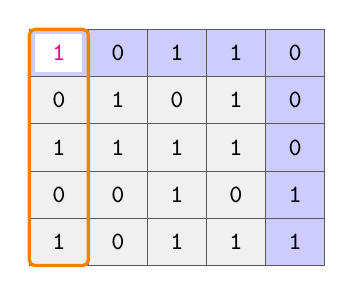
\begin{tikzpicture}[x=.75cm,y=.6cm,every node/.style={font=\small}]
                    \kartentrickGitter{0}
                    % c1 wird bei der Übertragung umgedreht
                    \fill<2->[white] (0.1,0.1) rectangle (0.9,0.9);
                    \node<2->[magenta,font=\small\bfseries\ttfamily] at (.5,.5) {1};
                    \draw<2->[orange,very thick,rounded corners=2pt] (0,-4) rectangle (1,1);
                \end{tikzpicture}
            \end{center}
        \end{column}
        \begin{column}{.55\textwidth}
            \begin{itemize}
                \item Ja: \(c_1\) prüft \(a_1,a_5,a_9,a_{13}\) \underline{und} sich selbst
                \item<2-> Beispiel: \(c_1\) kippt von \texttt{0} auf \texttt{1}
                \item<3-> Erste Spalte: \(\texttt{0}+\texttt{1}+\texttt{0}+\texttt{1}+\textcolor{magenta}{\texttt{1}}\), 3 Einsen $\rightarrow$ \(c_1\) meldet
                \item<3-> Sonst meldet nur \(c_9\) (zählt alle Bits)
                \item<4-> Kein \(a_i\) hat dieses Muster $\rightarrow$ \(c_1\) selbst ist gekippt
                \item<4-> Tabelle: Kreuz in Zeile \(c_1\), Spalte \(c_1\)
            \end{itemize}
        \end{column}
    \end{columns}
\end{frame}


% TikZ-Optionen nur auf bestimmten Folien anwenden, z.B. onslide=<1>{opacity=0}
\tikzset{onslide/.code args={<#1>#2}{\only<#1>{\pgfkeysalso{#2}}}}

\begin{frame}{Von der Tabelle zur Überwachungstabelle}
    \begin{center}
        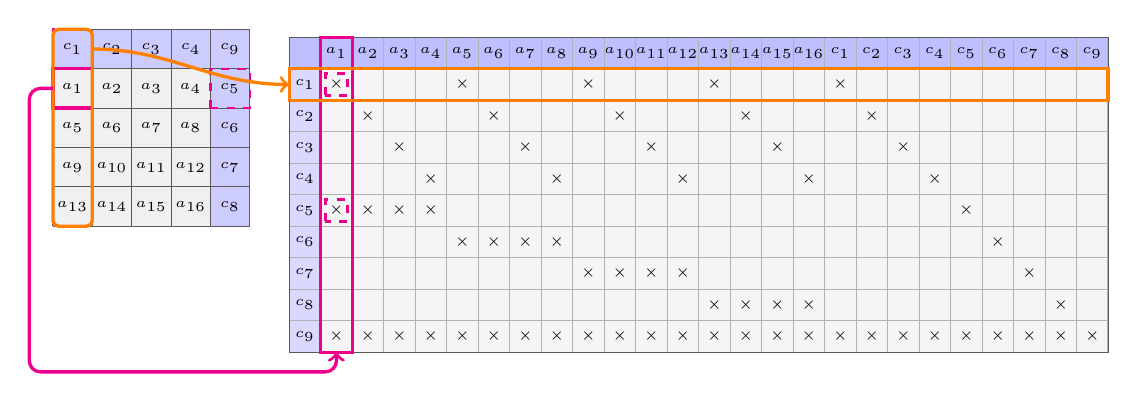
\begin{tikzpicture}[every node/.style={font=\tiny}]
            % links: Kartentrick-Tabelle mit den Namen der Bits
            \begin{scope}[x=.5cm,y=.5cm]
                \foreach \r in {1,...,4} {
                        \foreach \c in {1,...,4} {
                                \pgfmathtruncatemacro{\nr}{4*(\r-1)+\c}
                                \fill[gray!12] (\c-1,-\r) rectangle (\c,-\r+1);
                                \node at (\c-.5,-\r+.5) {\(a_{\nr}\)};
                            }
                    }
                \foreach \c in {1,...,4} {
                        \fill[blue!20] (\c-1,0) rectangle (\c,1);
                        \node at (\c-.5,.5) {\(c_{\c}\)};
                    }
                \foreach \r in {1,...,4} {
                        \pgfmathtruncatemacro{\nr}{\r+4}
                        \fill[blue!20] (4,-\r) rectangle (5,-\r+1);
                        \node at (4.5,-\r+.5) {\(c_{\nr}\)};
                    }
                \fill[blue!20] (4,0) rectangle (5,1);
                \node at (4.5,.5) {\(c_9\)};
                \draw[step=1,black!65] (0,-4) grid (5,1);
                % a1 liegt in der Spalte von c1 und in der Zeile von c5
                \draw<2>[magenta,very thick] (0,-1) rectangle (1,0);
                \draw<2>[magenta,thick,dashed] (0,0) rectangle (1,1);
                \draw<2>[magenta,thick,dashed] (4,-1) rectangle (5,0);
                \coordinate (g-a1) at (0,-.5);
                % Bereich von c1: die erste Spalte
                \draw<3>[orange,very thick,rounded corners=2pt] (0,-4) rectangle (1,1);
                \coordinate (g-c1) at (1,.5);
            \end{scope}
            % rechts: Überwachungstabelle, erst ab Schritt 2 sichtbar (Platz bleibt reserviert, damit nichts springt)
            \begin{scope}[x=.4cm,y=.4cm,shift={(3cm,0)},onslide=<1>{opacity=0}]
                \kartentrickUeberwachung
                % Spalte von a1: Kreuze bei c1, c5, c9
                \draw<2>[magenta,very thick] (1,-9) rectangle (2,1);
                % dieselben Kontrollbits c1 und c5 wie links gestrichelt
                \draw<2>[magenta,thick,dashed] (1.15,-.85) rectangle (1.85,-.15);
                \draw<2>[magenta,thick,dashed] (1.15,-4.85) rectangle (1.85,-4.15);
                \coordinate (t-a1) at (1.5,-9);
                % Zeile von c1: a1, a5, a9, a13 und c1
                \draw<3>[orange,very thick] (0,-1) rectangle (26,0);
                \coordinate (t-c1) at (0,-.5);
            \end{scope}
            % Pfeil links um die Kartentrick-Tabelle herum zur Spalte von a1
            \draw<2>[->,magenta,very thick,rounded corners=4pt] (g-a1) -- (-.3cm,-.25cm) -- (-.3cm,-3.85cm) -| (t-a1);
            \draw<3>[->,orange,very thick] (g-c1) to[out=0,in=180] (t-c1);
        \end{tikzpicture}
    \end{center}
    \begin{itemize}
        \item<2-> \(a_1\) liegt in Spalte \(c_1\) und Zeile \(c_5\), \(c_9\) zählt alles $\rightarrow$ Spalte \(a_1\): \(c_1, c_5, c_9\)
        \item<3-> \(c_1\) prüft die erste Spalte $\rightarrow$ Zeile \(c_1\): \(a_1, a_5, a_9, a_{13}, c_1\)
    \end{itemize}
\end{frame}


\begin{frame}{Überwachungstabelle}
    \begin{center}
        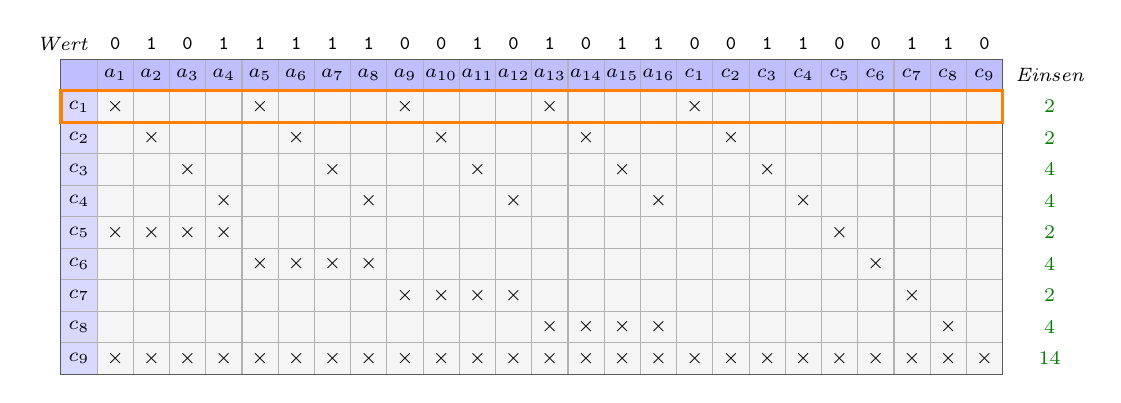
\begin{tikzpicture}[x=.46cm,y=.4cm,every node/.style={font=\scriptsize}]
            \kartentrickUeberwachung
            % Beispielcodewort über der Tabelle
            \uncover<2->{\kartentrickWertzeile{0}}
            % Anzahl Einsen unter den Kreuzen jeder Zeile
            \uncover<3->{
                \node[font=\scriptsize\itshape] at (27.3,.5) {Einsen};
                \foreach \n [count=\i] in {2,2,4,4,2,4,2,4,14} {
                        \node[green!50!black] at (27.3,.5-\i) {\n\ \checkmark};
                    }
            }
            % Zeile von c1 als Beispiel
            \draw<3->[orange,very thick] (0,-1) rectangle (26,0);
        \end{tikzpicture}
    \end{center}
    \begin{itemize}
        \item Zeile: Kontrollbit, Spalte: Bit des Codeworts, Kreuz: wird überwacht
        \item<3-> Zeile \(c_1\): unter den Kreuzen steht \texttt{0,1,0,1,0} $\rightarrow$ 2 Einsen
        \item<4-> In jeder Zeile gerade: die \tib{Anzahl Einsen unter den Kreuzen} (die Anzahl Kreuze ist egal)
    \end{itemize}
\end{frame}


\begin{frame}{Signatur eines Bits}
    \begin{center}
        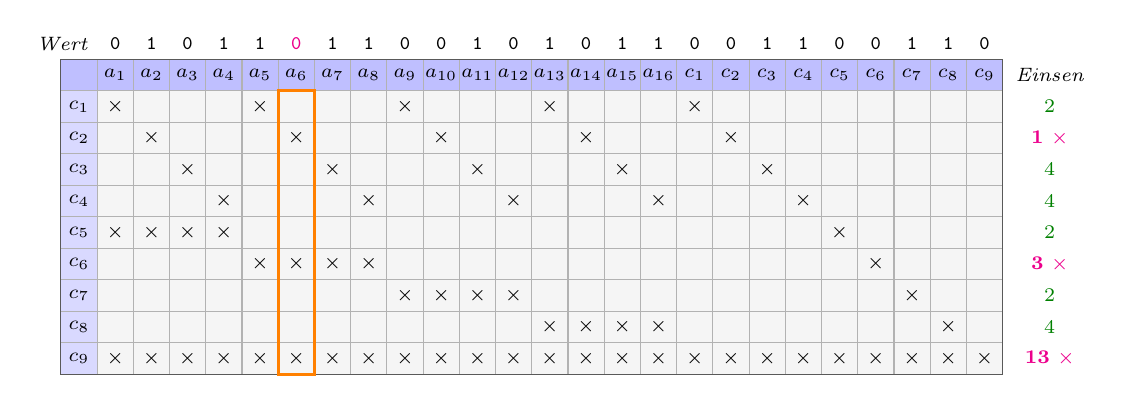
\begin{tikzpicture}[x=.46cm,y=.4cm,every node/.style={font=\scriptsize}]
            \kartentrickUeberwachung
            % a6 ist bei der Übertragung umgekippt
            \kartentrickWertzeile{6}
            \node[font=\scriptsize\itshape] at (27.3,.5) {Einsen};
            \foreach \n/\ok [count=\i] in {2/1,1/0,4/1,4/1,2/1,3/0,2/1,4/1,13/0} {
                    \ifnum\ok=1
                        \node[green!50!black] at (27.3,.5-\i) {\n\ \checkmark};
                    \else
                        \node<2->[magenta] at (27.3,.5-\i) {\textbf{\n}\ \(\boldsymbol{\times}\)};
                    \fi
                }
            % Spalte von a6: genau die meldenden Kontrollbits
            \draw<3->[orange,very thick] (6,-9) rectangle (7,0);
        \end{tikzpicture}
    \end{center}
    \begin{columns}[onlytextwidth]
        \begin{column}{.3\textwidth}
            \begin{center}
                % Kartentrick-Tabelle vom Anfang mit gekipptem a6
                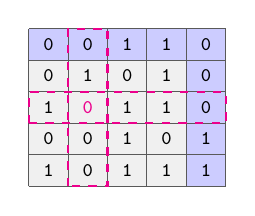
\begin{tikzpicture}[x=.5cm,y=.4cm,every node/.style={font=\scriptsize}]
                    \kartentrickGitter{6}
                    % Spalte von c2 und Zeile von c6 melden
                    \draw<2->[magenta,thick,dashed] (1,-4) rectangle (2,1);
                    \draw<2->[magenta,thick,dashed] (0,-2) rectangle (5,-1);
                \end{tikzpicture}
            \end{center}
        \end{column}
        \begin{column}{.55\textwidth}
            \begin{itemize}
                \item Empfangen: \(a_6\) ist von \texttt{1} auf \textcolor{magenta}{\texttt{0}} gekippt
                \item<2-> Ungerade, melden also: \(c_2, c_6, c_9\)
                \item<3-> Spalte \(a_6\): Kreuze genau bei \(c_2, c_6, c_9\)
                \item<4-> \tib{Signatur} eines Bits: seine Spalte, also wer bei seinem Fehler meldet
            \end{itemize}
        \end{column}
        % Platz für das Logo unten rechts
        \begin{column}{.15\textwidth}
        \end{column}
    \end{columns}
\end{frame}


\begin{frame}{Wann ist eine Codierung 1-fehlerkorrigierend?}
    \begin{myremark}[Merksatz]
        Eine Codierung ist genau dann 1-fehlerkorrigierend, wenn die Spalten ihrer Überwachungstabelle
        \begin{itemize}
            \item paarweise verschieden und
            \item nicht leer sind.
        \end{itemize}
    \end{myremark}
    \pause
    \begin{itemize}[<+->]
        \item Gleiche Spalten: Zwei Bits haben dieselbe Signatur $\rightarrow$ Fehler nicht lokalisierbar.\\
              Beispiel: Hätte \(a_2\) wie \(a_6\) die Signatur \(c_2, c_6, c_9\), wüsste man beim obigen Fehler nicht, ob \(a_2\) oder \(a_6\) gekippt ist
        \item Leere Spalte: Ein Fehler in diesem Bit wird nie bemerkt
        \item Kartentrick: Auch ohne \(c_9\) bleiben alle Spalten verschieden und nicht leer $\rightarrow$ 8 Kontrollbits genügen.\\
              Beispiel: \(a_6\) hätte dann die Signatur \(c_2, c_6\)
    \end{itemize}
\end{frame}


\begin{frame}{Wie viele Kontrollbits sind mindestens nötig?}
    \begin{columns}[T,onlytextwidth]
        \begin{column}{.42\textwidth}
            \begin{center}
                % alle 2^3 = 8 möglichen Spalten bei n = 3 Kontrollbits
                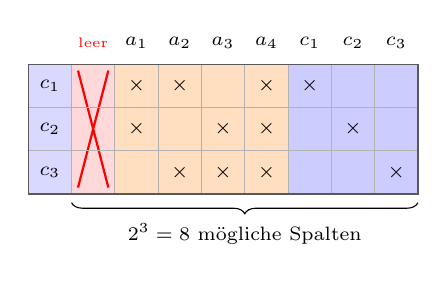
\begin{tikzpicture}[x=.55cm,y=.55cm,every node/.style={font=\scriptsize}]
                    \fill[blue!15] (0,-3) rectangle (1,0);
                    \fill[gray!8] (1,-3) rectangle (9,0);
                    \foreach \i in {1,2,3} {
                            \node at (.5,.5-\i) {\(c_{\i}\)};
                        }
                    % Muster der Spalten (Zeilen c1, c2, c3): leer, a1 bis a4, c1 bis c3
                    % führende 1 nur, damit pgfmath z.B. 011 nicht als Oktalzahl liest
                    \foreach \muster [count=\col] in {1000,1110,1101,1011,1111,1100,1010,1001} {
                            \foreach \z in {1,2,3} {
                                    \pgfmathtruncatemacro{\bit}{mod(floor(\muster/10^(3-\z)),10)}
                                    \ifnum\bit=1
                                        \node at (\col+.5,.5-\z) {\(\times\)};
                                    \fi
                                }
                        }
                    % die leere Spalte ist verboten
                    \fill<2->[red!15] (1,-3) rectangle (2,0);
                    \draw<2->[red,thick] (1.15,-2.85) -- (1.85,-.15) (1.15,-.15) -- (1.85,-2.85);
                    \node<2->[red,font=\tiny] at (1.5,.5) {leer};
                    % die Kontrollbits brauchen je eine Spalte
                    \fill<3->[blue!20] (6,-3) rectangle (9,0);
                    \foreach \i in {1,2,3} {
                            \pgfmathtruncatemacro{\col}{5+\i}
                            \node<3-> at (\col+.5,.5-\i) {\(\times\)};
                            \node<3-> at (\col+.5,.5) {\(c_{\i}\)};
                        }
                    % die übrigen Spalten bleiben für die Nachrichtenbits
                    \fill<4->[orange!25] (2,-3) rectangle (6,0);
                    \foreach \muster [count=\i] in {1110,1101,1011,1111} {
                            \pgfmathtruncatemacro{\col}{1+\i}
                            \node<4-> at (\col+.5,.5) {\(a_{\i}\)};
                            \foreach \z in {1,2,3} {
                                    \pgfmathtruncatemacro{\bit}{mod(floor(\muster/10^(3-\z)),10)}
                                    \ifnum\bit=1
                                        \node<4-> at (\col+.5,.5-\z) {\(\times\)};
                                    \fi
                                }
                        }
                    \draw[step=1,black!30,thin] (0,-3) grid (9,0);
                    \draw[black!65] (0,-3) rectangle (9,0);
                    \draw[decorate,decoration={brace,mirror,amplitude=4pt}] (1,-3.2) -- (9,-3.2)
                    node[midway,below=4pt] {\(2^3=8\) mögliche Spalten};
                \end{tikzpicture}
            \end{center}
        \end{column}
        \begin{column}{.55\textwidth}
            \begin{itemize}[<+->]
                \item \(K=3\) Kontrollbits $\rightarrow$ 3 Zeilen, jede Zelle mit oder ohne Kreuz $\rightarrow$ \(2^3=8\) mögliche Spalten
                \item Die leere Spalte ist verboten $\rightarrow$ \(2^3-1=7\) nutzbare Spalten
                \item Die Kontrollbits brauchen 3 davon
                \item Bleiben 4 Spalten für Nachrichtenbits: \(N+K = 4+3 \leq 7\)
                \item Allgemein: \(K\) Kontrollbits, \(N\) Nachrichtenbits
                      \[
                          2^K-1 \geq N+K
                      \]
            \end{itemize}
        \end{column}
    \end{columns}
\end{frame}


\begin{frame}{Wie viele Kontrollbits braucht eine 16-Bit-Nachricht?}
    \begin{center}
        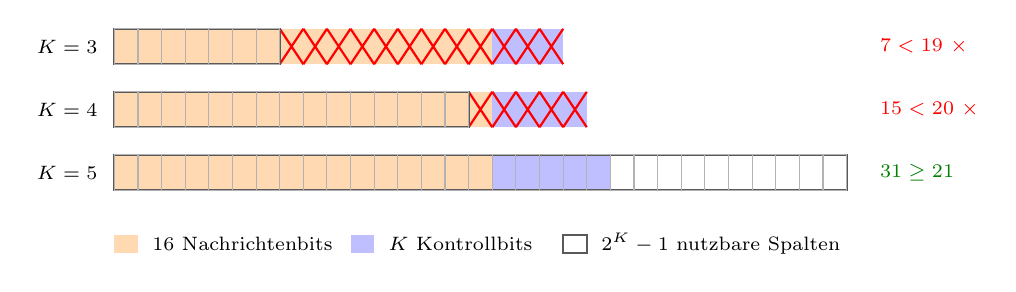
\begin{tikzpicture}[x=.3cm,y=.45cm,every node/.style={font=\scriptsize}]
            % je Zeile: verfügbare Spalten (grau umrandet) und benötigte Spalten (16 a + K c)
            \foreach \n [count=\z] in {3,4,5} {
                    \pgfmathtruncatemacro{\frei}{2^\n-1}
                    \pgfmathtruncatemacro{\noetig}{16+\n}
                    \begin{scope}[yshift=-\z*.8cm]
                        \node[anchor=east] at (-.3,.5) {\(K=\n\)};
                        \uncover<\z->{
                            % benötigte Spalten: Nachrichtenbits und Kontrollbits
                            \foreach \i in {1,...,\noetig} {
                                    \ifnum\i>16
                                        \fill[blue!25] (\i-1,0) rectangle (\i,1);
                                    \else
                                        \fill[orange!30] (\i-1,0) rectangle (\i,1);
                                    \fi
                                }
                            % nicht genug verfügbare Spalten: Überschuss rot
                            \ifnum\noetig>\frei
                                \pgfmathtruncatemacro{\ab}{\frei+1}
                                \foreach \i in {\ab,...,\noetig} {
                                        \draw[red,thick] (\i-1,0) -- (\i,1) (\i-1,1) -- (\i,0);
                                    }
                            \fi
                            \draw[black!65,thick] (0,0) rectangle (\frei,1);
                            \foreach \i in {1,...,\frei} {
                                    \draw[black!30] (\i-1,0) rectangle (\i,1);
                                }
                            \ifnum\noetig>\frei
                                \node[anchor=west,red] at (32,.5) {\(\frei < \noetig\) \(\times\)};
                            \else
                                \node[anchor=west,green!50!black] at (32,.5) {\(\frei \geq \noetig\) \checkmark};
                            \fi
                        }
                    \end{scope}
                }
            % Legende
            \fill[orange!30] (0,-7.1) rectangle (1,-6.6);
            \node[anchor=west] at (1.2,-6.85) {16 Nachrichtenbits};
            \fill[blue!25] (10,-7.1) rectangle (11,-6.6);
            \node[anchor=west] at (11.2,-6.85) {\(K\) Kontrollbits};
            \draw[black!65,thick] (19,-7.1) rectangle (20,-6.6);
            \node[anchor=west] at (20.2,-6.85) {\(2^K-1\) nutzbare Spalten};
        \end{tikzpicture}
    \end{center}
    \begin{itemize}
        \item<4-> Mindestens \underline{5 Kontrollbits} (statt 9 beim Kartentrick)
    \end{itemize}
\end{frame}


\begin{frame}{Optimale Überwachungstabelle für 16 Bit}
    \begin{center}
        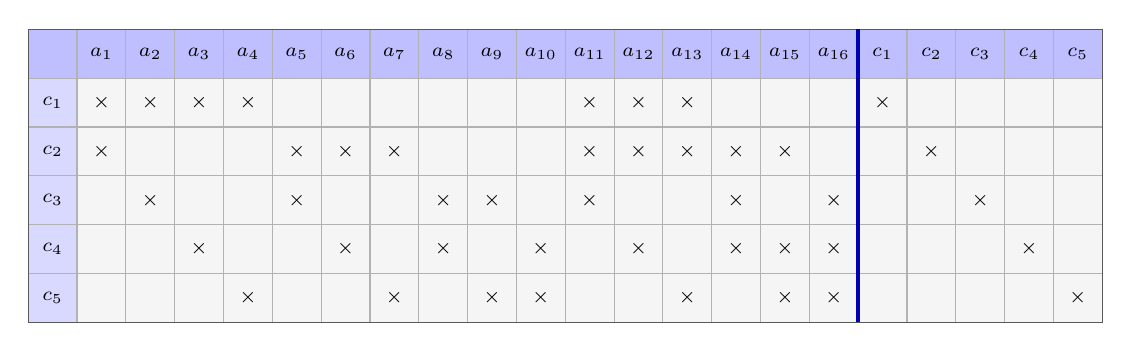
\begin{tikzpicture}[x=.62cm,y=.62cm,every node/.style={font=\scriptsize}]
            % Hintergrund
            \fill[blue!25] (0,0) rectangle (22,1);
            \fill[blue!15] (0,-5) rectangle (1,0);
            \fill[gray!8] (1,-5) rectangle (22,0);
            % Spalten- und Zeilenbeschriftung
            \foreach \i in {1,...,16} {
                    \node at (\i+.5,.5) {\(a_{\i}\)};
                }
            \foreach \i in {1,...,5} {
                    \pgfmathtruncatemacro{\col}{16+\i}
                    \node at (\col+.5,.5) {\(c_{\i}\)};
                    \node at (.5,.5-\i) {\(c_{\i}\)};
                }
            % Überwachungsbereiche der Nachrichtenbits (wie im Skript)
            \foreach \col in {1,2,3,4,11,12,13} {
                    \node at (\col+.5,-.5) {\(\times\)};
                }
            \foreach \col in {1,5,6,7,11,12,13,14,15} {
                    \node at (\col+.5,-1.5) {\(\times\)};
                }
            \foreach \col in {2,5,8,9,11,14,16} {
                    \node at (\col+.5,-2.5) {\(\times\)};
                }
            \foreach \col in {3,6,8,10,12,14,15,16} {
                    \node at (\col+.5,-3.5) {\(\times\)};
                }
            \foreach \col in {4,7,9,10,13,15,16} {
                    \node at (\col+.5,-4.5) {\(\times\)};
                }
            % Kontrollbits überwachen sich selbst
            \foreach \i in {1,...,5} {
                    \pgfmathtruncatemacro{\col}{16+\i}
                    \node at (\col+.5,.5-\i) {\(\times\)};
                }
            \draw[step=1,black!30,thin] (0,-5) grid (22,1);
            \draw[black!65] (0,-5) rectangle (22,1);
            % Trennung Nachrichtenbits / Kontrollbits
            \draw[blue!70!black,very thick] (17,-5) -- (17,1);
        \end{tikzpicture}
    \end{center}
    \begin{itemize}[<+->]
        \item Kontrollbits: je ein Kreuz in der eigenen Zeile
        \item Nachrichtenbits: Kreuze frei wählbar, solange alle Spalten verschieden und nicht leer sind
        \item Codewort: 16 + 5 = 21 Bit
        \item Beispiel: Die Spalte von \(a_6\) hat Kreuze bei \(c_2\) und \(c_4\). Diese Signatur kommt beim Decodieren wieder vor
    \end{itemize}
\end{frame}


\begin{frame}{Codieren}
    Nachricht: \texttt{0101 1111 0010 1011}
    \begin{itemize}[<+->]
        \item \(c_1\) überwacht \(a_1, a_2, a_3, a_4, a_{11}, a_{12}, a_{13}\):
              \texttt{\textcolor{orange}{0101} 1111 00\textcolor{orange}{10 1}011}\\
              Anzahl Einsen gerade $\rightarrow$ \(c_1 = 0\)
        \item \(c_2\) überwacht \(a_1, a_5, a_6, a_7, a_{11}, \ldots, a_{15}\):
              \texttt{\textcolor{orange}{0}101 \textcolor{orange}{111}1 00\textcolor{orange}{10 101}1}\\
              Anzahl Einsen gerade $\rightarrow$ \(c_2 = 0\)
        \item Ebenso: \(c_3 = 1\), \(c_4 = 0\), \(c_5 = 1\)
        \item Codewort:
              \[
                  \underbrace{\texttt{0101 1111 0010 1011}}_{\text{Nachricht}}
                  \ \underbrace{\texttt{00101}}_{\text{Kontrollbits}}
              \]
    \end{itemize}
\end{frame}


\begin{frame}{Decodieren: Fehler finden}
    Empfangen: \texttt{0101 1\textcolor{magenta}{0}11 0010 1011 00101}
    \begin{itemize}[<+->]
        \item Für jedes Kontrollbit prüfen: Ist die Anzahl Einsen im Überwachungsbereich (samt Kontrollbit) gerade?
        \item Verletzt: \(c_2\) und \(c_4\). In Ordnung: \(c_1, c_3, c_5\)
        \item Signatur \((c_1, \ldots, c_5) = (\cdot, \times, \cdot, \times, \cdot)\)
        \item Die einzige Spalte mit dieser Signatur ist \(a_6\)
        \item \(a_6\) umdrehen: \texttt{0101 1\textcolor{orange}{1}11 0010 1011 00101}
    \end{itemize}
\end{frame}


% Beispiel mit 4 Nachrichtenbits und 3 Kontrollbits (optimale Überwachungstabelle, 2^3 - 1 = 4 + 3)
% Farben der Kontrollbits
\colorlet{ueA}{orange!90!black}
\colorlet{ueB}{teal}
\colorlet{ueC}{violet}
% Überwachungsbereiche als Positionen im Codewort a1 a2 a3 a4 c1 c2 c3
\def\bereichA{1,2,4,5}
\def\bereichB{1,3,4,6}
\def\bereichC{2,3,4,7}

% Überwachungstabelle direkt über dem Codewort: jede Tabellenspalte steht über ihrem Bit
\newcommand{\vierBitGrund}{%
    % Codewort-Kästchen (Namen stehen in der Kopfzeile der Tabelle)
    \foreach \i in {1,...,4} {
            \fill[gray!12] (\i-.4,-.4) rectangle (\i+.4,.4);
        }
    \foreach \i in {5,6,7} {
            \fill[blue!15] (\i-.4,-.4) rectangle (\i+.4,.4);
        }
    \foreach \i in {1,...,7} {
            \draw[black!50] (\i-.4,-.4) rectangle (\i+.4,.4);
        }
    % Tabellenhintergrund wie bei den anderen Überwachungstabellen
    \fill[blue!25] (-.5,2.1) rectangle (7.5,2.6);
    \fill[blue!15] (-.5,.6) rectangle (.5,2.1);
    \fill[gray!8] (.5,.6) rectangle (7.5,2.1);
    % Spalten- und Zeilenbeschriftung
    \foreach \i/\n in {1/a_1,2/a_2,3/a_3,4/a_4,5/c_1,6/c_2,7/c_3} {
            \node at (\i,2.35) {\(\n\)};
        }
    \node[ueA] at (0,1.85) {\(c_1\)};
    \node[ueB] at (0,1.35) {\(c_2\)};
    \node[ueC] at (0,.85) {\(c_3\)};
    % Kreuze in der Farbe des Kontrollbits
    \foreach \i in \bereichA {\node[ueA,font=\bfseries] at (\i,1.85) {\(\times\)};}
    \foreach \i in \bereichB {\node[ueB,font=\bfseries] at (\i,1.35) {\(\times\)};}
    \foreach \i in \bereichC {\node[ueC,font=\bfseries] at (\i,.85) {\(\times\)};}
    % Gitter: Spaltenmitten liegen auf ganzen Zahlen, die Linien dazwischen
    \foreach \x in {.5,1.5,...,6.5} {\draw[black!30,thin] (\x,.6) -- (\x,2.6);}
    \foreach \y in {1.1,1.6,2.1} {\draw[black!30,thin] (-.5,\y) -- (7.5,\y);}
    \draw[black!65] (-.5,.6) rectangle (7.5,2.6);
    % Trennung Nachrichtenbits / Kontrollbits
    \draw[blue!70!black,very thick] (4.5,.6) -- (4.5,2.6);
    % feste Grösse, damit die Grafik zwischen den Animationsschritten nicht springt
    \path[use as bounding box] (-.6,-3.8) rectangle (9.2,2.7);
}

% #1 = Farbe, #2 = Bereich, #3 = y-Mitte der Tabellenzeile: Zeile einfärben und Kästchen des Bereichs umranden
\newcommand{\vierBitBereich}[3]{%
    \fill[#1,opacity=.15] (.5,#3-.25) rectangle (7.5,#3+.25);
    \foreach \i in #2 {
            \draw[#1,ultra thick] (\i-.4,-.4) rectangle (\i+.4,.4);
        }
}


\begin{frame}{Beispiel: Kontrollbits für \texttt{1011} berechnen}
    \begin{center}
        \begin{tikzpicture}[x=1.2cm,y=1cm,every node/.style={font=\small}]
            \vierBitGrund
            % zuerst der Bereich (Farbe), erst im nächsten Schritt die Zahl
            \only<2-3>{\vierBitBereich{ueA}{\bereichA}{1.85}}
            \only<4-5>{\vierBitBereich{ueB}{\bereichB}{1.35}}
            \only<6-7>{\vierBitBereich{ueC}{\bereichC}{.85}}
            \foreach \i/\v in {1/1,2/0,3/1,4/1} {
                    \node[font=\large\ttfamily] at (\i,0) {\v};
                }
            \node<1-2>[gray] at (5,0) {?};
            \node<1-4>[gray] at (6,0) {?};
            \node<1-6>[gray] at (7,0) {?};
            \node<3->[ueA,font=\large\ttfamily\bfseries] at (5,0) {0};
            \node<5->[ueB,font=\large\ttfamily\bfseries] at (6,0) {1};
            \node<7->[ueC,font=\large\ttfamily\bfseries] at (7,0) {0};
            % Einsen im Bereich ohne das Kontrollbit, dann auf gerade ergänzen
            \node<3->[anchor=west,ueA] at (.6,-1.3) {\(c_1\): \texttt{1+0+1} = 2 Einsen \(\rightarrow\) \(c_1 = \texttt{0}\)};
            \node<5->[anchor=west,ueB] at (.6,-1.85) {\(c_2\): \texttt{1+1+1} = 3 Einsen \(\rightarrow\) \(c_2 = \texttt{1}\)};
            \node<7->[anchor=west,ueC] at (.6,-2.4) {\(c_3\): \texttt{0+1+1} = 2 Einsen \(\rightarrow\) \(c_3 = \texttt{0}\)};
            \node<8->[anchor=west] at (.6,-3.1) {Codewort: \texttt{1011\,\underline{010}}};
        \end{tikzpicture}
    \end{center}
\end{frame}


\begin{frame}{Beispiel: Ein Bit kippt}
    \begin{center}
        \begin{tikzpicture}[x=1.2cm,y=1cm,every node/.style={font=\small}]
            \vierBitGrund
            % zuerst der Bereich (Farbe), erst im nächsten Schritt das Ergebnis
            \only<3-4>{\vierBitBereich{ueA}{\bereichA}{1.85}}
            \only<5-6>{\vierBitBereich{ueB}{\bereichB}{1.35}}
            \only<7-8>{\vierBitBereich{ueC}{\bereichC}{.85}}
            \foreach \i/\v in {1/1,2/0,4/1,5/0,6/1,7/0} {
                    \node[font=\large\ttfamily] at (\i,0) {\v};
                }
            % a3 kippt von 1 auf 0 und wird am Schluss zurückgekippt
            \node<1>[font=\large\ttfamily] at (3,0) {1};
            \node<2-9>[magenta,font=\large\ttfamily\bfseries] at (3,0) {0};
            \node<10->[green!50!black,font=\large\ttfamily\bfseries] at (3,0) {1};
            % meldende Kontrollbits markieren
            \draw<6->[magenta,thick] (0,1.35) circle (.22);
            \draw<8->[magenta,thick] (0,.85) circle (.22);
            % Signatur: die Tabellenspalte von a3 hat Kreuze genau bei c2 und c3
            \draw<9->[magenta,very thick,rounded corners=2pt] (2.55,.55) rectangle (3.45,2.65);
            \node<2->[anchor=west,magenta] at (.6,-1.3) {\(a_3\) kippt: \texttt{10\textbf{0}1\,\underline{010}}};
            \node<4->[anchor=west,ueA] at (.6,-1.85) {\(c_1\): \texttt{1+0+1+0} = 2, gerade \textcolor{green!50!black}{\checkmark}};
            \node<6->[anchor=west,ueB] at (.6,-2.4) {\(c_2\): \texttt{1+0+1+1} = 3, ungerade \(\rightarrow\) \(c_2\) meldet};
            \node<8->[anchor=west,ueC] at (.6,-2.95) {\(c_3\): \texttt{0+0+1+0} = 1, ungerade \(\rightarrow\) \(c_3\) meldet};
            \node<9->[anchor=west] at (.6,-3.6) {Signatur \textcolor{ueB}{\(c_2\)}, \textcolor{ueC}{\(c_3\)}: nur die Spalte von \(a_3\) \(\rightarrow\) \(a_3\) zurückkippen};
        \end{tikzpicture}
    \end{center}
\end{frame}


\begin{frame}{Auftrag}{Skript \enquote{Datenintegrität}}
    \begin{itemize}
        \item Abschnitt 1.6 bis und mit \enquote{Konstruktion einer optimalen Überwachungstabelle} lesen
        \item \aufgabebox{1.19, 1.20 (Anzahl Kontrollbits), 1.22 (Codieren und Decodieren)}
        \item \challengebox{1.21 (Codierung entwerfen)}
    \end{itemize}
\end{frame}


\begin{frame}{Richard Hamming (1915--1998)}
    \begin{columns}
        \begin{column}{.48\textwidth}
            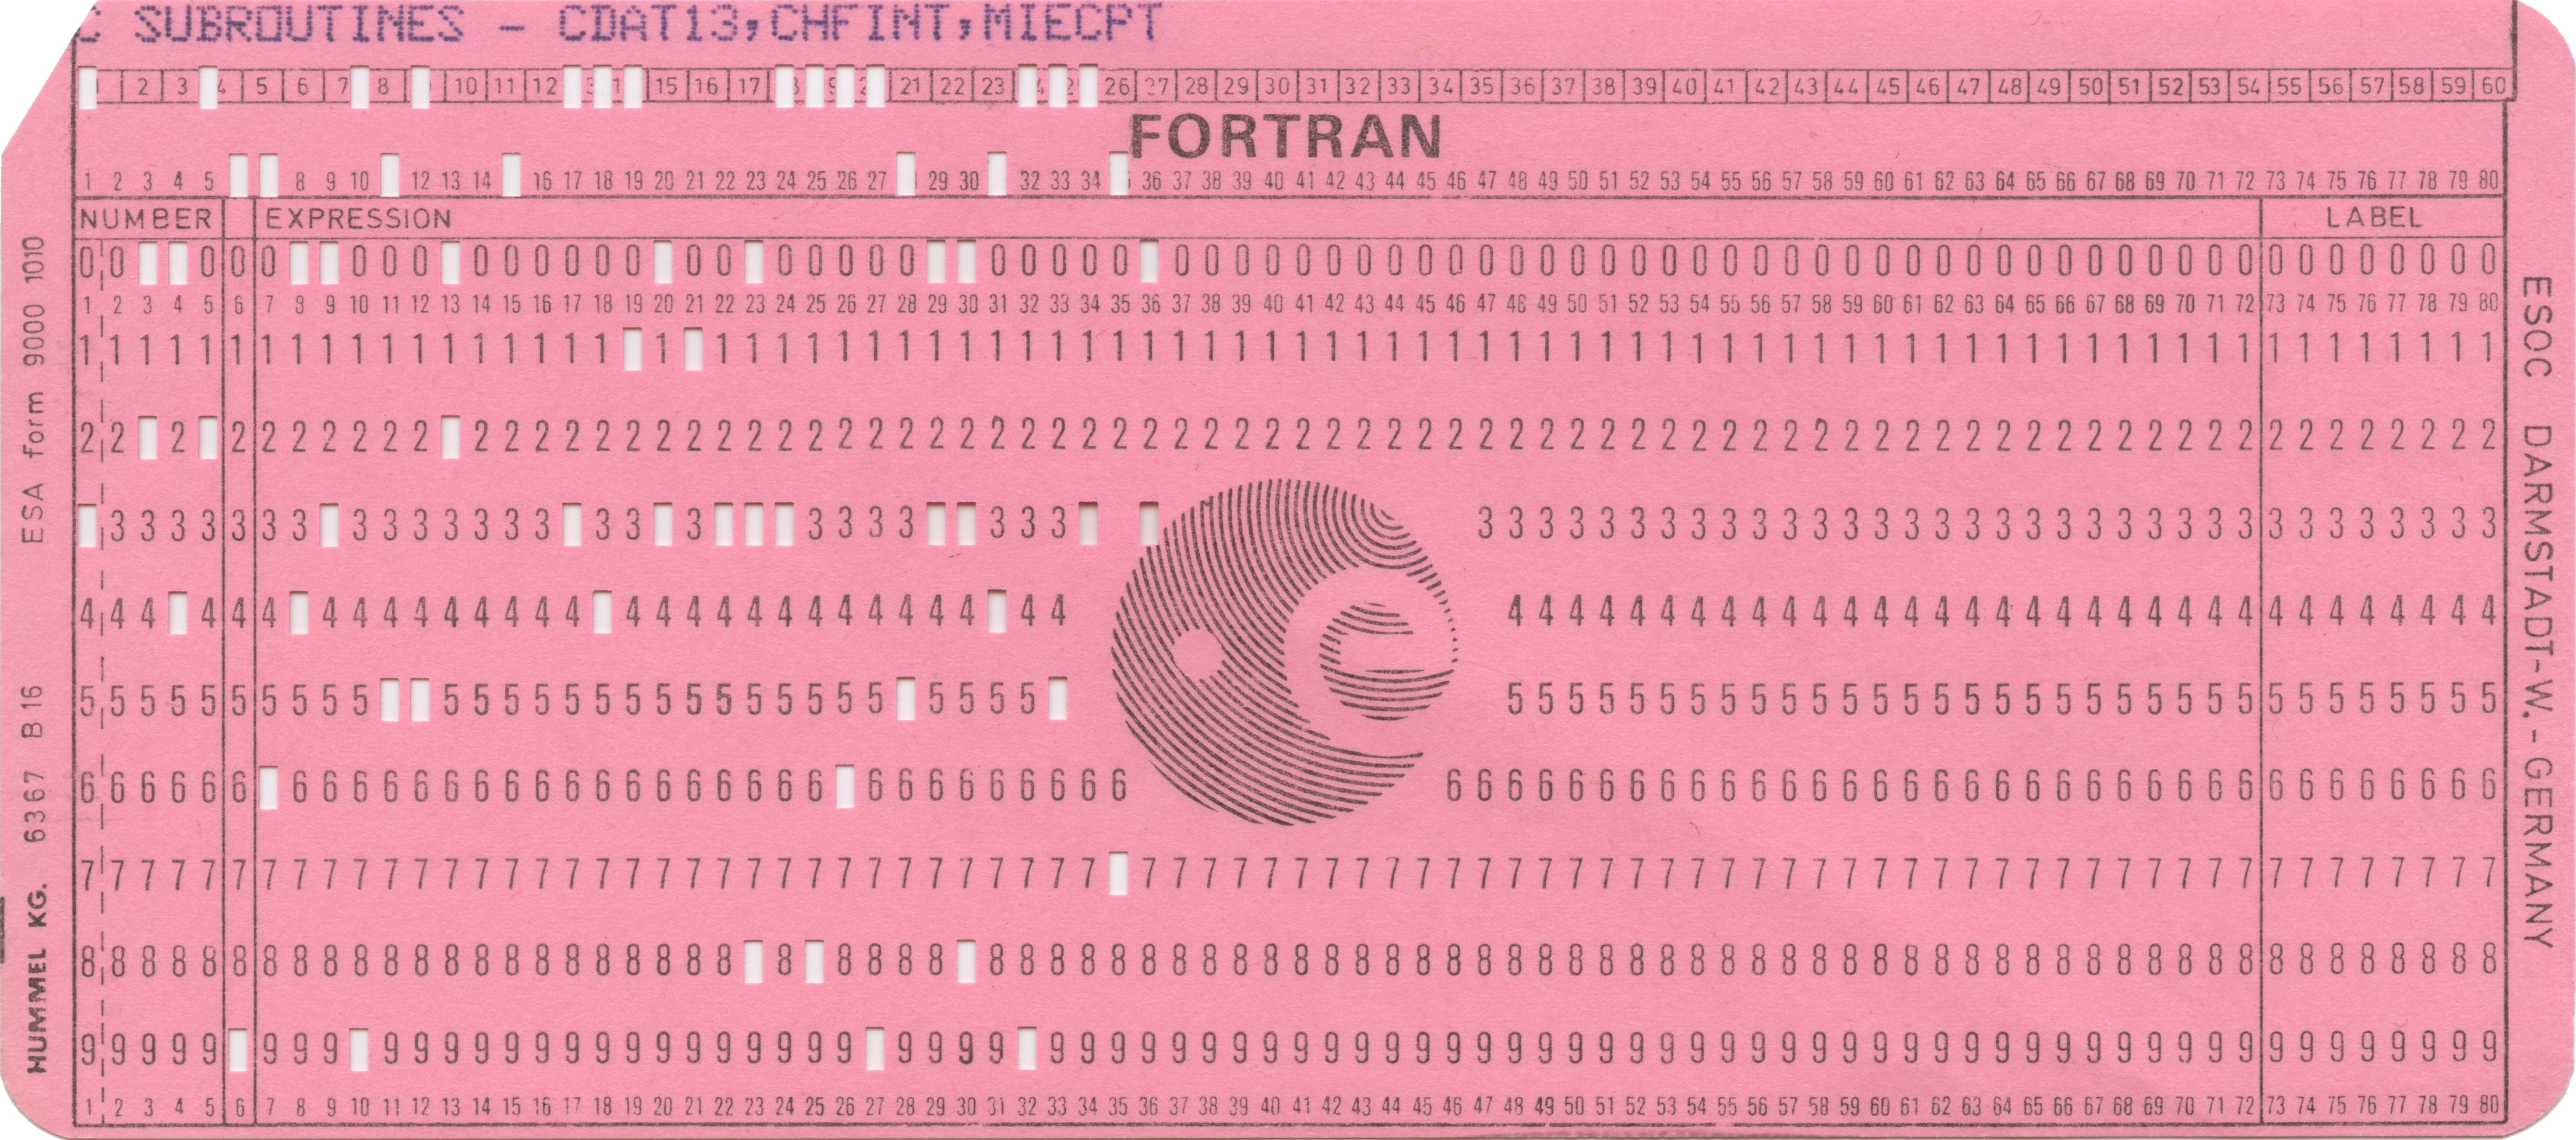
\includegraphics[width=\linewidth]{Grundlagen_Info/05_Datenintegritaet/Figures/Fortran_punch_card_ESA.jpg}\\
            {\tiny Fortran-Lochkarte der ESA, 70er Jahre. Till Niermann, CC BY-SA 3.0, via \href{https://commons.wikimedia.org/wiki/File:Fortran_punch_card_ESA.jpg}{Wikimedia Commons}}
        \end{column}
        \begin{column}{.48\textwidth}
            \begin{itemize}[<+->]
                \item Mathematiker bei den Bell Laboratories
                \item Programme und Daten auf Lochkarten: Loch = 1, kein Loch = 0
                \item Lesefehler wurden oft erst nach langer Rechenzeit bemerkt
                \item Hamming-Codes (1950): einzelne Bitfehler mit wenigen Kontrollbits korrigieren
            \end{itemize}
        \end{column}
    \end{columns}
\end{frame}


\begin{frame}{Hamming-Codes: Kontrollbits an Zweierpotenz-Positionen}
    \begin{columns}
        \begin{column}{.42\textwidth}
            \begin{center}
                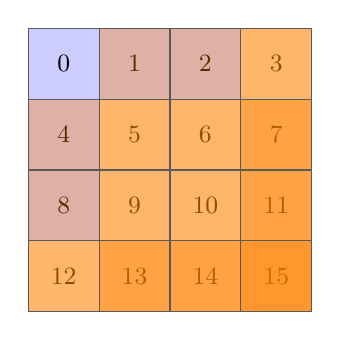
\begin{tikzpicture}[x=.9cm,y=.9cm,every node/.style={font=\small}]
                    % Positionen 0 bis 15 im 4x4-Raster
                    \foreach \p in {0,...,15} {
                            \pgfmathtruncatemacro{\col}{mod(\p,4)}
                            \pgfmathtruncatemacro{\row}{div(\p,4)}
                            \node at (\col+.5,-\row-.5) {\p};
                        }
                    % Kontrollbits hervorheben
                    \foreach \p in {0,1,2,4,8} {
                            \pgfmathtruncatemacro{\col}{mod(\p,4)}
                            \pgfmathtruncatemacro{\row}{div(\p,4)}
                            \fill[blue!20] (\col,-\row) rectangle (\col+1,-\row-1);
                            \node at (\col+.5,-\row-.5) {\p};
                        }
                    % Überwachungsbereiche nacheinander einblenden
                    \fill<2>[orange,opacity=.35] (1,0) rectangle (2,-4) (3,0) rectangle (4,-4);
                    \fill<3>[orange,opacity=.35] (2,0) rectangle (4,-4);
                    \fill<4>[orange,opacity=.35] (0,-1) rectangle (4,-2) (0,-3) rectangle (4,-4);
                    \fill<5>[orange,opacity=.35] (0,-2) rectangle (4,-4);
                    \draw[step=1,black!65] (0,0) grid (4,-4);
                \end{tikzpicture}
            \end{center}
        \end{column}
        \begin{column}{.55\textwidth}
            \begin{itemize}
                \item 16 Bit: 11 Nachrichtenbits, Kontrollbits an den Positionen 1, 2, 4, 8 (und 0)
                \item<2-> Position 1 überwacht die 2.\ und 4.\ Spalte
                \item<3-> Position 2 überwacht die 3.\ und 4.\ Spalte
                \item<4-> Position 4 überwacht die 2.\ und 4.\ Zeile
                \item<5-> Position 8 überwacht die 3.\ und 4.\ Zeile
                \item<6-> Die verletzten Kontrollbits ergeben die Fehlerposition, z.\,B.\ 1 und 4 verletzt $\rightarrow$ Position \(1+4=5\)
                \item<7-> Position 0: Parität über alles, erkennt zusätzlich zwei Fehler
            \end{itemize}
        \end{column}
    \end{columns}
\end{frame}


\begin{frame}{Auftrag}{Skript \enquote{Datenintegrität}}
    \begin{itemize}
        \item Beispiel 1.8 (Hamming-Code) im Skript durchgehen
        \item \aufgabebox{1.23 (Hamming-Code)}
    \end{itemize}
\end{frame}


\begin{frame}{Geht es mit noch weniger Bits? Der Hyperwürfel}
    \begin{columns}
        \begin{column}{.45\textwidth}
            \begin{center}
                \begin{tikzpicture}
                    \HyperCube{3}
                \end{tikzpicture}
            \end{center}
        \end{column}
        \begin{column}{.5\textwidth}
            \begin{itemize}[<+->]
                \item Punkt: Bitfolge der Länge \(L\)
                \item Kante: Die Bitfolgen unterscheiden sich in genau einem Bit
                \item Ein Bitfehler $=$ ein Schritt entlang einer Kante
            \end{itemize}
        \end{column}
    \end{columns}
\end{frame}


\begin{frame}{Zonen eines 1-fehlerkorrigierenden Codes}
    \begin{columns}
        \begin{column}{.45\textwidth}
            \begin{center}
                \begin{tikzpicture}
                    \HyperCube{3}
                    \only<2->{\CircleNodes[orange,double]{hg-011}}
                    \only<3->{\CircleNodes[orange]{hg-001,hg-010,hg-111}}
                    \only<4->{
                        \CircleNodes[green,double]{hg-100}
                        \CircleNodes[green]{hg-000,hg-110,hg-101}
                    }
                \end{tikzpicture}
            \end{center}
        \end{column}
        \begin{column}{.5\textwidth}
            \begin{itemize}
                \item<2-> Codewort \texttt{011} (doppelter Kreis)
                \item<3-> Seine \textcolor{orange}{Zone}: Codewort und seine \(L\) Nachbarn
                \item<4-> Zweites Codewort \texttt{100} mit \textcolor{green!60!black}{Zone}. Zonen dürfen sich nicht überlappen
                \item<5-> Die Zonen füllen den Würfel lückenlos aus: Der Code ist \tib{perfekt}
            \end{itemize}
        \end{column}
    \end{columns}
\end{frame}


\begin{frame}{Hamming-Codes sind perfekt}
    \begin{itemize}[<+->]
        \item Hamming-Code ohne Position 0: 15 Bit, davon 11 Nachrichtenbits
        \item \(2^{11}=2048\) Codewörter, jede Zone hat \(15+1=16\) Punkte
        \item \(2048\cdot 16=2^{15}\): Die Zonen füllen den Hyperwürfel lückenlos aus
        \item Kein Platz für ein weiteres Codewort, der Code lässt sich nicht verbessern
    \end{itemize}
\end{frame}


\begin{frame}{Auftrag}{Skript \enquote{Datenintegrität}}
    \begin{itemize}
        \item \aufgabebox{1.24, 1.25 (Hyperwürfel)}
    \end{itemize}
\end{frame}
